% !TeX root = ../../Parte1.tex
\secmeme{html/select}
\section{Form}

\begin{frame}[fragile]{Form}\transfade\centering
  \htmlDual[-s A7][][trim={0 6cm 0 0},clip]{<meta charset="utf-8">}{
<form>
    <label> Username: </label>
    <input type="text" placeholder="Username">
    <br>
    <label> E-mail: </label>
    <input type="email" placeholder="user@mail.it">
    <br>
    <label> Password: </label>
    <input type="password">
    <br>
    <input type="submit" value="Registrati">
</form>
  }{<script>document.getElementsByTagName('input')[2].value="1234"</script>}
\end{frame}
\begin{frame}[fragile]{Form}\transfade\centering
  \begin{columns}
    \begin{column}{.56\textwidth}
      \begin{minted}[breaklines]{html}
<form>
    <label> Username: </label>
    <input type="text" id="user_field" name="user" placeholder="Username">
    <br>
    <label> E-mail: </label>
    <input type="email" id="mail_field" name="mail" placeholder="user@mail.it">
    <br>
    <label> Password: </label>
    <input type="password" id="pass_field" name="pass">
    <br>
    <input type="submit" value="Registrati">
</form>
      \end{minted}
    \end{column}
    \hfill
    \begin{column}{.42\textwidth}
      \makeatletter
      \includegraphics[width=\textwidth,trim={0 7cm 0 0},clip]{\html@dir/\jobname _\thehtml@count.pdf}
      \makeatother
    \end{column}
  \end{columns}
  \bigskip
  L'attributo \mintattribute{name} da un nome al campo \minttag{input} per poterne elaborare i dati.\\
\end{frame}
\begin{frame}[fragile]{Form}\transfade\centering
  \begin{columns}
    \begin{column}{.56\textwidth}
      \begin{minted}[breaklines]{html}
<form>
    <label for="user_field"> Username: </label>
    <input type="text" id="user_field" name="user" placeholder="Username">
    <br>
    <label for="mail_field"> E-mail: </label>
    <input type="email" id="mail_field" name="mail" placeholder="user@mail.it">
    <br>
    <label for="pass_field"> Password: </label>
    <input type="password" id="pass_field" name="pass">
    <br>
    <input type="submit" value="Registrati">
</form>
      \end{minted}
    \end{column}
    \hfill
    \begin{column}{.42\textwidth}
      \makeatletter
      \includegraphics[width=\textwidth,trim={0 7cm 0 0},clip]{\html@dir/\jobname _\thehtml@count.pdf}
      \makeatother
    \end{column}
  \end{columns}
  \bigskip
  I \minttag{label} sono utili per l'accessibilità del sito e vanno collegati all'\minttag{input} corretto impostando l'attributo \mintattribute{for} come l'\mintattribute{id} dell'\minttag{input}.\\
\end{frame}

\begin{frame}[fragile]{Radio button}\transfade\centering
  \htmlDual[-s A7][breaklines][trim={0 8cm 0 0},clip]{<meta charset="utf-8">}{
<form>
    <p> HTML è </p>

    <input type="radio" id ="facile" name="difficulty" value="0">
    <label for="facile"> Facile </label>
    <br>
    <input type="radio" id ="difficile" name="difficulty" value="10">
    <label for="difficile"> Difficile </label>
</form>
  }{<script>document.getElementById('facile').checked=true</script>}
\end{frame}

\begin{frame}[fragile]{Checkbox}\transfade\centering
  \htmlDual[-s A7][breaklines][trim={0 8cm 0 0},clip]{<meta charset="utf-8">}{
<form>
    <p> HTML è </p>

    <input type="checkbox" id ="stupendo" name="html" value="beatiful">
    <label for="stupendo"> Stupendo </label>
    <br>
    <input type="checkbox" id ="facile" name="html" value="easy">
    <label for="facile"> Facile </label>
    <br>
    <input type="checkbox" id ="difficile" name="html" value="difficult">
    <label for="difficile"> Difficile </label>
</form>
  }{<script>document.getElementById('facile').checked=true;document.getElementById('stupendo').checked=true</script>}
\end{frame}

\begin{frame}[fragile]{Valori di defualt}\transfade\centering
  \htmlDual[-s A7][breaklines][trim={0 7cm 0 0},clip]{<meta charset="utf-8">}{
<form>
    <label for="nome"> Nome: </label>
    <input type="text" id="nome" name="name" placeholder="Inserisci il tuo nome"  value="Pinco Pallino">

    <p> HTML è </p>

    <input type="checkbox" id ="stupendo" name="html" value="beatiful" checked>
    <label for="stupendo"> Stupendo </label>
    <br>
    <input type="checkbox" id ="difficile" name="html" value="difficult">
    <label for="difficile"> Difficile </label>
</form>
  }{}
\end{frame}

\begin{frame}[fragile]{Altri attributi}\transfade\centering
  \htmlDual[-s A7][breaklines][trim={0 8cm 0 0},clip]{<meta charset="utf-8">}{
<form>
    <label for="nome"> Nome: </label>
    <input type="text" id="nome" name="name" placeholder="Inserisci il tuo nome" value="Pinco" disabled>
    <br>
    <label for="cognome"> Cognome: </label>
    <input type="text" id="cognome" name="surname" placeholder="Inserisci il tuo cognome" value="Pallino" readonly>
    <br>
    <input type="checkbox" id="consenso" name="accept" required>
    <label for="consenso"> Accetto le condizioni </label>
</form>
  }{}\bigskip
  \begin{description}
    \item[\mintattribute{disabled}] Non modificabile e non considerato durante l'elaborazione dei dati.
    \item[\mintattribute{readonly}] Non modificabile, ma considerato durante l'elaborazione dei dati.
    \item[\mintattribute{required}]<2-> La compilazione del campo è obbligatria.
  \end{description}
\end{frame}

\begin{frame}[fragile]{Menù a tendina}\transfade\centering
  \htmlDual[-s A7][breaklines][trim={0 8cm 0 0},clip]{<meta charset="utf-8">}{
<form>
    <label for="numero"> Scegli un numero: </label>
    <select id="numero" name="number">
        <option value="0"> Zero </option>
        <option value="1" selected> Uno </option>
        <option value="2"> Due </option>
    </select>
</form>
  }{}
\end{frame}

\begin{frame}[fragile]{Scelta multipla}\transfade\centering
  \htmlDual[-s A7][breaklines][trim={0 8cm 0 0},clip]{<meta charset="utf-8"><style>#numeri{height:65px}</style>}{
<form>
    <label for="numeri"> Scegli dei numeri: </label><br>
    <select id="numeri" name="numbers" size="3" multiple>
        <option value="0"> Zero </option>
        <option value="1" selected> Uno </option>
        <option value="2" selected> Due </option>
        <option value="3"> Tre </option>
    </select>
</form>
  }{}
\end{frame}

\begin{frame}[fragile]{Altri elementi}\transfade\centering
  \htmlDual[-s A7][breaklines][trim={0 6cm 0 0},clip]{<meta charset="utf-8"><style>#numeri{height:65px}</style>}{
<form>
    <textarea name="commento" rows="3" cols="30">
        Inserisci il tuo commento...
    </textarea>
    <br>
    <input type="number" min="0" max="9" value="8">
    <br>
    <input type="date" min="1970-01-01" max="2070-01-01" value="2018-07-22">
    <br>
    <button type="button"> Cliccami </button>
</form>
  }{<script>document.getElementsByName('commento')[0].innerHTML="Inserisci il tuo commento...";document.getElementsByTagName('input')[1].value="22 Luglio 2018"</script>}
\end{frame}

\begin{frame}\transfade
  \begin{exercise}\centering
    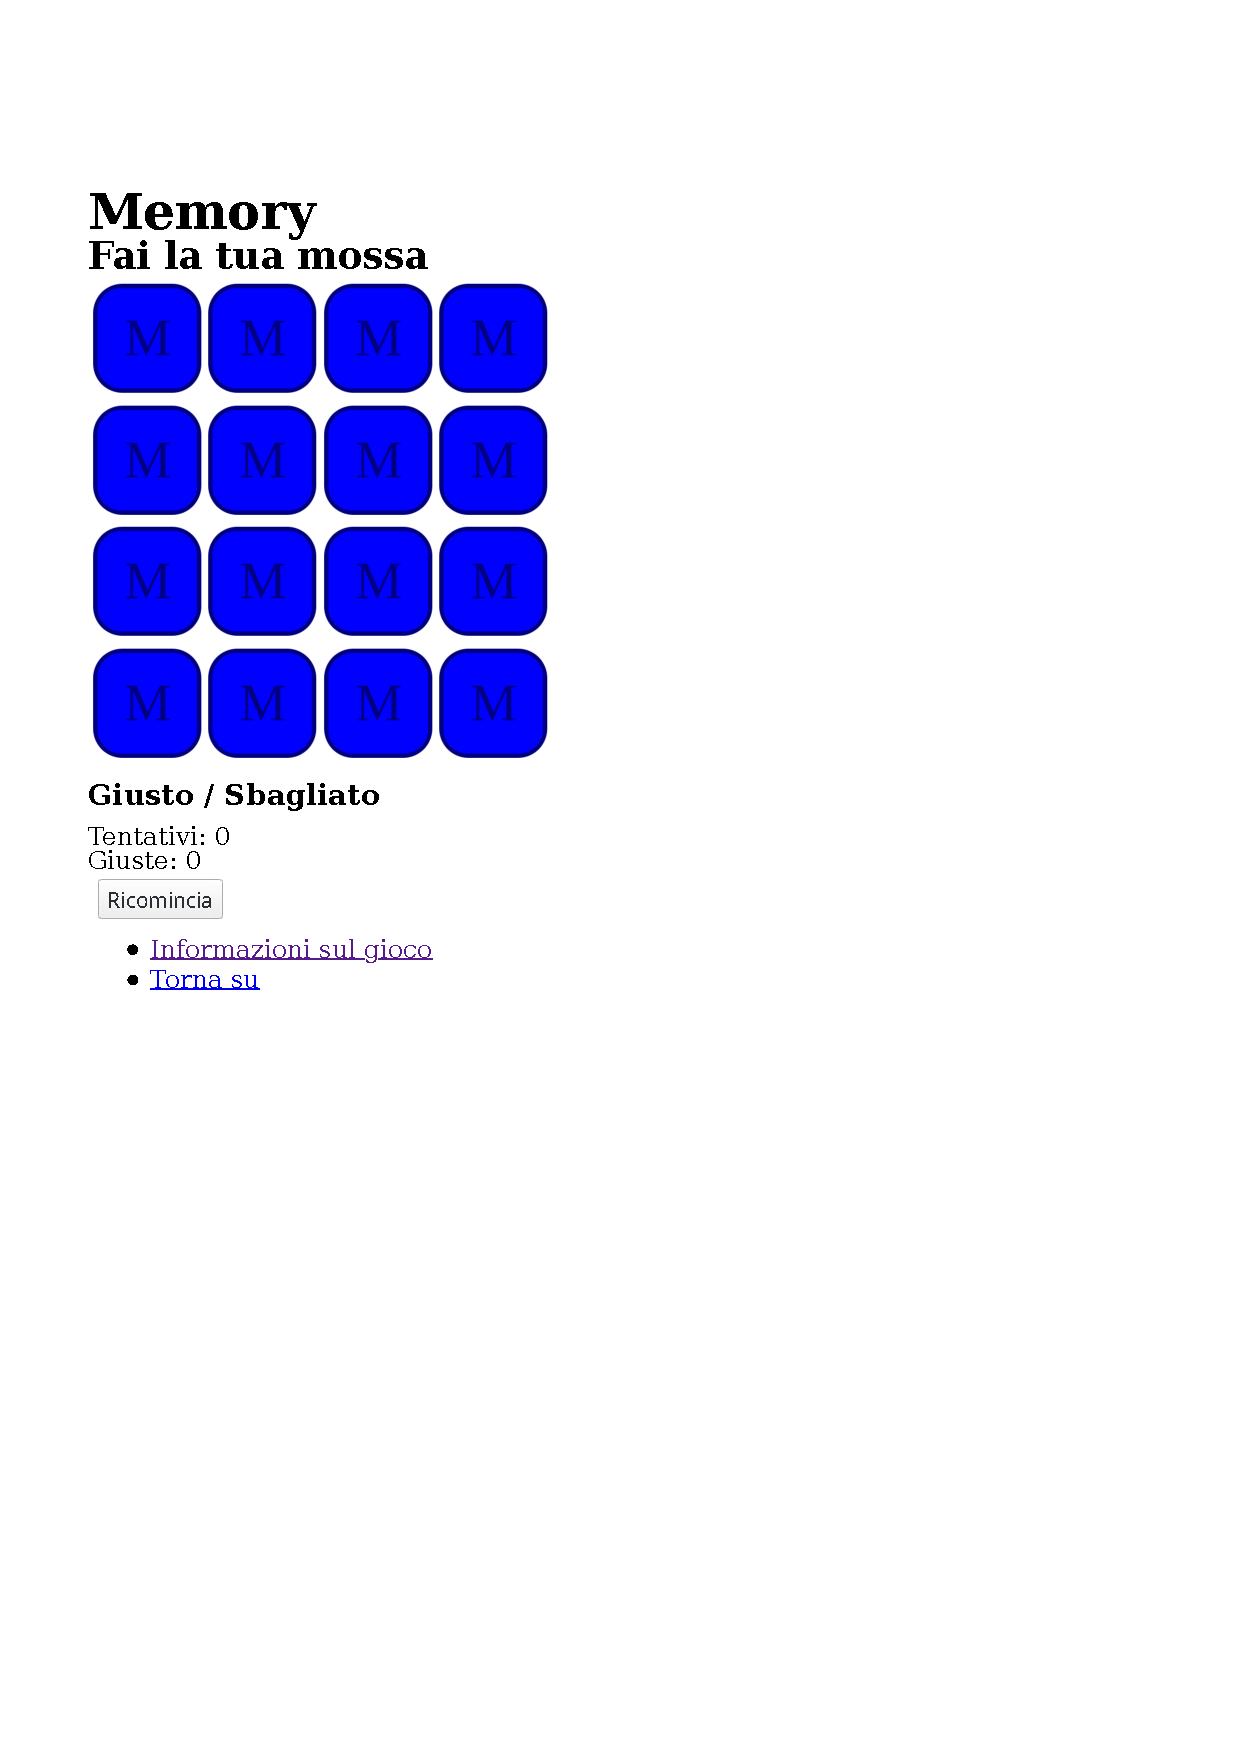
\includegraphics[height=.85\textheight]{memory/html/memory.pdf}
  \end{exercise}
\end{frame}

\begin{frame}[fragile]\transfade
  \begin{sol}\centering
    \begin{minted}{html}
<button> Ricomincia </button>
    \end{minted}
  \end{sol}
\end{frame}